\documentclass{beamer}

\usepackage{enumitem}
\usepackage{pgfplots}

\usetheme{Boadilla}
\title{Fourier Transformation}
\subtitle{Using Beamer}
\author{Gourove Roy}
\institute{Department of CSE, BUET}
\date{\today}

\begin{document}

\begin{frame}
    \titlepage
\end{frame}

\begin{frame}
    \frametitle{Introduction to Fourier Transforms}
    \begin{itemize}[label=$\star$, itemsep=15pt, parsep=0pt, topsep=10pt]
        \item Fourier transform
        \item Inverse Fourier transform: The Fourier integral theorem
        \item The rect and sinc functions
        \item Cosine and Sine Transforms
        \item Symmetry properties
        \item Periodic signals and $\delta$ functions
    \end{itemize}
\end{frame}

\begin{frame}
    \frametitle{Fourier Transforms}
    Given a continuous time signal $x(t)$, de ne its Fourier transform as the
 function of a real $f, X(f)\footnote{Usually $X(f)$ is written as $X(i2\pi f)$ or $X(i\omega)$. This corresponds to
 the Laplace transform notation which we encountered when discussing
 transfer functions $H(s)$.}$ is :
    \begin{equation*}
        X(f) = \int_{-\infty}^{\infty} x(t) e^{-j2\pi ft} dt
    \end{equation*}
    This is similar to the expression for the Fourier series coefficients.
\end{frame}

\begin{frame}
    \frametitle{Inverse Fourier Transforms}
    Continuous-time Fourier Transform yields the \emph{inversion formula} for the Fourier transform, the \emph{Fourier
 integral theorem}:
    \begin{equation*}
        X(f) = \int_{-\infty}^{\infty} x(t) e^{-j2\pi ft} dt
    \end{equation*}
    \begin{equation*}
        x(t) = \int_{-\infty}^{\infty} X(f) e^{j2\pi ft} df
    \end{equation*}
    The Fourier transform and its inverse are symmetric in the sense that the Fourier
    transform of $x(t)$ is $X(f)$ and the Fourier transform of $X(f)$ is $x(-t)$. This is
    a consequence of the symmetry of the complex exponential.
\end{frame}

\begin{frame}
    \frametitle{Cosine and Sine Transforms}
    Assume x(t) is a possibly complex signal.
    \begin{equation*}
        \begin{split}
            X(f) &= \int_{-\infty}^{\infty} x(t) e^{-j2\pi ft} dt\\
            &= \int_{-\infty}^{\infty} x(t) \cos(2\pi ft) dt - j\int_{-\infty}^{\infty} x(t) \sin(2\pi ft) dt\\
            &= \int_{-\infty}^{\infty} x(t) \cos(\omega t) dt - j\int_{-\infty}^{\infty} x(t) \sin(\omega t) dt
        \end{split}
    \end{equation*}
\end{frame}

\begin{frame}
    \frametitle{Fourier Transform Notation}
    For convenience, we will write the Fourier transform of a signal $x(t)$ as
    \begin{equation*}
        X(f) = \mathcal{F}\{x(t)\}
    \end{equation*}
    and the inverse Fourier transform of $X(f)$ as
    \begin{equation*}
        x(t) = \mathcal{F}^{-1}\{X(f)\}
    \end{equation*}
    Note that
    \begin{equation*}
        \mathcal{F}^{-1}\{\mathcal{F}\{x(t)\}\} = x(t)
    \end{equation*}
    at points of continuity of x(t).
\end{frame}

\begin{frame}
    \frametitle{The rect and sinc functions}
    The Fourier transform of a rectangular pulse is a sinc function and the Fourier transform of a sinc function is a rectangular pulse.
    \begin{equation*}
        x(t) = \text{rect}(t) = \begin{cases}
            1 & \text{if } |t| < \frac{1}{2}\\
            0 & \text{otherwise}
        \end{cases}
    \end{equation*}
    \begin{equation*}
        X(f) = \text{sinc}(f) = \begin{cases}
            1 & \text{if } |f| < \frac{1}{2}\\
            0 & \text{otherwise}
        \end{cases}
    \end{equation*}
    Note that the sinc function is defined as $\text{sinc}(f) = \frac{\sin(\pi f)}{\pi f}$.
\end{frame}

\begin{frame}
    \frametitle{rect and sinc function graphs}
    \begin{minipage}{0.45\textwidth} % Reduced width
        \begin{tikzpicture}[scale=0.9] % Scale down the plot
            \begin{axis}[%
                axis lines=middle,
                xmin=-2, xmax=2,
                ymin=-0.5, ymax=1.5,
                xlabel={$t$}, ylabel={$\mathrm{rect}(t)$},
                xtick={-1, -0.5, 0, 0.5, 1},
                ytick={0, 1},
                domain=-2:2,
                samples=200
            ]
                \addplot[thick, blue] {abs(x) <= 0.5 ? 1 : 0};
            \end{axis}
        \end{tikzpicture}
    \end{minipage}
    \hspace{0.02\textwidth} % Add space between the graphs
    \begin{minipage}{0.45\textwidth} % Reduced width
        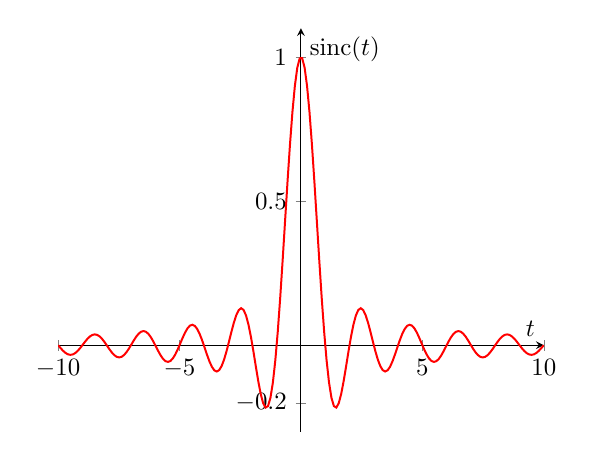
\begin{tikzpicture}[scale=0.9] % Scale down the plot
            \begin{axis}[%
                axis lines=middle,
                xmin=-10, xmax=10,
                ymin=-0.3, ymax=1.1,
                xlabel={$t$}, ylabel={$\mathrm{sinc}(t)$},
                xtick={-10, -5, 0, 5, 10},
                ytick={-0.2, 0, 0.5, 1},
                domain=-10:10,
                samples=200
            ]
                \addplot[thick, red, samples=200, domain=-10:10] 
                    {(x == 0) ? 1 : sin(deg(pi*x))/(pi*x)};
            \end{axis}
        \end{tikzpicture}
    \end{minipage}
\end{frame}

\begin{frame}
    \frametitle{Duality}
    Notice that the Fourier transform \mathcal{F} and the inverse Fourier transform
    \mathcal{F} are almost the same.
\end{frame}

\end{document}
